\documentclass[../defence.tex]{subfiles}

\begin{document}

  \begin{frame}{Kelvin equation}
        $-\left( \frac{1}{R_1}+ \frac{1}{R_2}\right) V_\mathrm{mol}^\mathrm{l} = RT \ln \frac{P_\mathrm{v}}{P_\mathrm{sv}}$ \\
        \pause

        $P_\mathrm{sp} = P_\mathrm{sv}\cdot \exp \left( - \frac{\gamma V_\mathrm{mol}^\mathrm{l}}{R_0\cdot RT}\right)< P_\mathrm{sv}$ \\
        \pause

        $P_\mathrm{eq} = P_\mathrm{sv}\cdot \exp \left( - \frac{2\cdot \gamma V_\mathrm{mol}^\mathrm{l}}{R_0\cdot RT}\right) < P_\mathrm{sp} < P_\mathrm{sv}$
        \pause

        \scalebox{0.55}{
          %\tikzsetnextfilename{kelvin_equation_plot}
          \tikzexternaldisable
          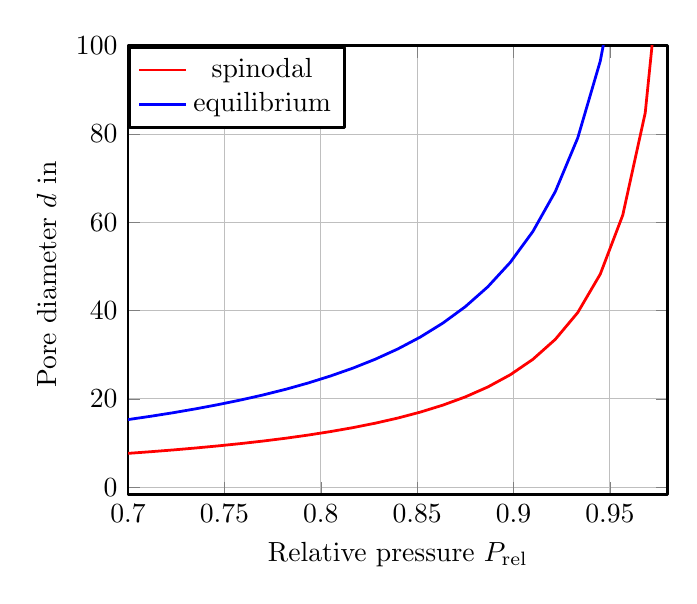
\begin{tikzpicture}
            \def\R{8.3144598}     %
            \def\gamma{0.018605}  % newton per meter
            \def\T{19+273.15} % kelvin
            \def\Vm{0.13053}  % litre per mol
              \begin{axis}[
                /tikz/line join=bevel,
                grid,
                legend style={at={(0,1)}, legend columns=1, anchor=north west},
                every axis plot,
      					line width = 1pt,
      					%	minor x tick num= ,
      					%	minor y tick num= ,
      					xmin = 0.7, xmax = 0.98,
      					ymax = 100,
      					xlabel = {Relative pressure $P_\mathrm{rel}$},
      					ylabel = {Pore diameter $d$ in $\si{\nano\meter}$},
                ]
                  \addplot[domain=0.7:0.98, red]
                    {- (2 * \gamma * \Vm / \R / \T / 100 ) / ln(x)};
                  \addlegendentry{spinodal}
                  \addplot[domain=0.7:0.98, blue]
                    {- 2*(2 * \gamma * \Vm / \R / \T / 100 ) / ln(x)};
                  \addlegendentry{equilibrium}
                \end{axis}
          \end{tikzpicture}}
  \end{frame}

\end{document}
